\documentclass[../summary.tex]{subfiles}

\begin{document}
	
\section{Biodiversity}
\subsection{What is biodiversity and where does it come from?}
\subsubsection{What is biodiversity?}

Biodiversity is a term that refers to the variety of life forms on Earth. Coined in 1985 by biologist Walter Rosen during the National Forum on Biodiversity. The term gained widespread use without a precise definition until the UN Convention on Biological Diversity in Rio de Janeiro, which provided a clear definition. \\
\\
Biodiversity was defined as "the variability among living organisms from all sources, including terrestrial, marine, and other aquatic ecosystems, and the ecological complexes of which they are parts."\\
\\
Biodiversity encompasses diversity within species, between species, and of ecosystems. It is measured at three levels: genetic diversity, species diversity, and ecosystem diversity. Genetic diversity refers to the variation among individuals within the same species. Species diversity is the number of known species at a particular location, with approximately 2.2 million species known in 2022. Ecosystem diversity encompasses a wide range of ecosystems, from forests to aquatic systems, contributing to the overall diversity on Earth.\\
\\
In 2011, it was estimated that in total, 8.8 million species live on the earth. This means that we still don't know 75\% of all living species today.

\subsubsection{Where does biodiversity come from?}

The history of life on Earth, with an estimated 8.7 million eukaryote species, is a story that spans billions of years. Understanding when and how these species appeared is made possible through the study of fossils, which provides insights into the emergence and extinction of various life forms. Key milestones include:

\begin{itemize}
	\item \textbf{Emergence of Life}: The Earth is approximately 4.5 billion years old. Bacterial life began around 3.7 billion years ago.
	\item \textbf{Cambrian Explosion}: Roughly 570 million years ago, the Cambrian explosion saw a rapid increase in species diversity, possibly due to rising oxygen levels.
	\item \textbf{Emergence of Life Forms}: Fish appeared 500 million years ago, land plants around 470 million years ago, and mammals roughly 200 million years ago.
	\item \textbf{Speciation}: The process behind the increasing species richness is speciation, which involves different populations of the same species evolving into distinct species, driven by natural selection.
	\item \textbf{Current Species}: Today's species represent only a fraction of all that have existed (between 2\% and 5\%).
	\item \textbf{Extinctions}: Extinctions have occurred throughout history, both gradually (background extinctions) and catastrophically (mass extinctions).
	\item \textbf{Mass Extinctions}: Five major mass extinctions, caused by events like meteorite impacts and volcanic activity, have occurred since the Cambrian. The most famous was the dinosaur-extinction event 65 million years ago, linked to a meteorite impact. The most severe was the Permian-Triassic extinction, where over 90\% of species disappeared.
\end{itemize}
\ \\
Recovery from mass extinctions has taken at least 10 million of years, underscoring the importance of preserving the diverse life on our planet.
\newpage

\subsection{Biodiversity loss and humans}
\subsubsection{Historical extinction}

The Late Quaternary or Pleistocene Megafaunal extinction wave, caused by human hunting, occurred around 60,000 years ago when Homo sapiens colonized the globe. This wave resulted in the extinction of large animals, such as the European lion and the giant sloths. The overkill hypothesis, developed by Paul Martin in the 1970s, suggests that human hunting caused the extinction of megafauna roaming the globe during the Pleistocene. \\
\\
Modern humans colonized the globe in four waves, with the last wave occurring less than 1000 years ago. The extinction of large mammals in Australia (almost 90\%) and Europe (35\%) coincided with the extinction of about 85\% of American megafauna. There is a striking parallel between timing of colonization by humans and extinctions. The effects of the extinction of one species can cascade throughout the entire food web.\\
\\
Comparing data on body size of animals that have gone extinct over 10,000 years ago reveals selective impact on larger animals, with small species escaping extinctions. Large mammals and top predators, like the elephant and lion, survived humans in Africa, possibly due to co-evolution and adaptation to hunting.

\subsubsection{Recent biodiversity loss}
\label{sec:recent-diversity-loss}
Humans had a strong hand in recent species extinctions. Since 1500, around 160 bird species, 60 mammal species and 100 species of other vertebrate groups, like reptiles and amphibians,  have been extinct. A famous example of an extinct species is the Dodo, as seen in figure \ref{fig:recentbiodiversityloss}.

\begin{figure}[H]
	\centering
	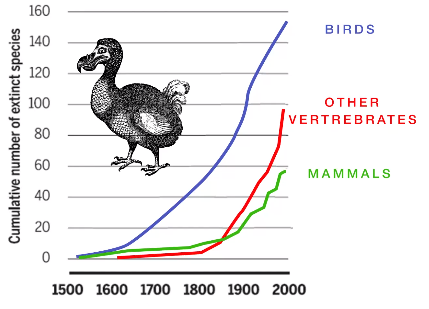
\includegraphics[width=0.6\linewidth]{../images/recent_biodiversity_loss}
	\caption{Cumulative number of extinct species since 1500}
	\label{fig:recentbiodiversityloss}
\end{figure}
\ \\

A lot of species are not extinct yet, but face strong declines in numbers.  

An example of this is the tiger, which occurred in large parts of Asia. But now, it has been pushed back to a small part of it's original range.  The global population declined by 50\% between 1998 and 2015.

\begin{figure}[H]
	\centering
	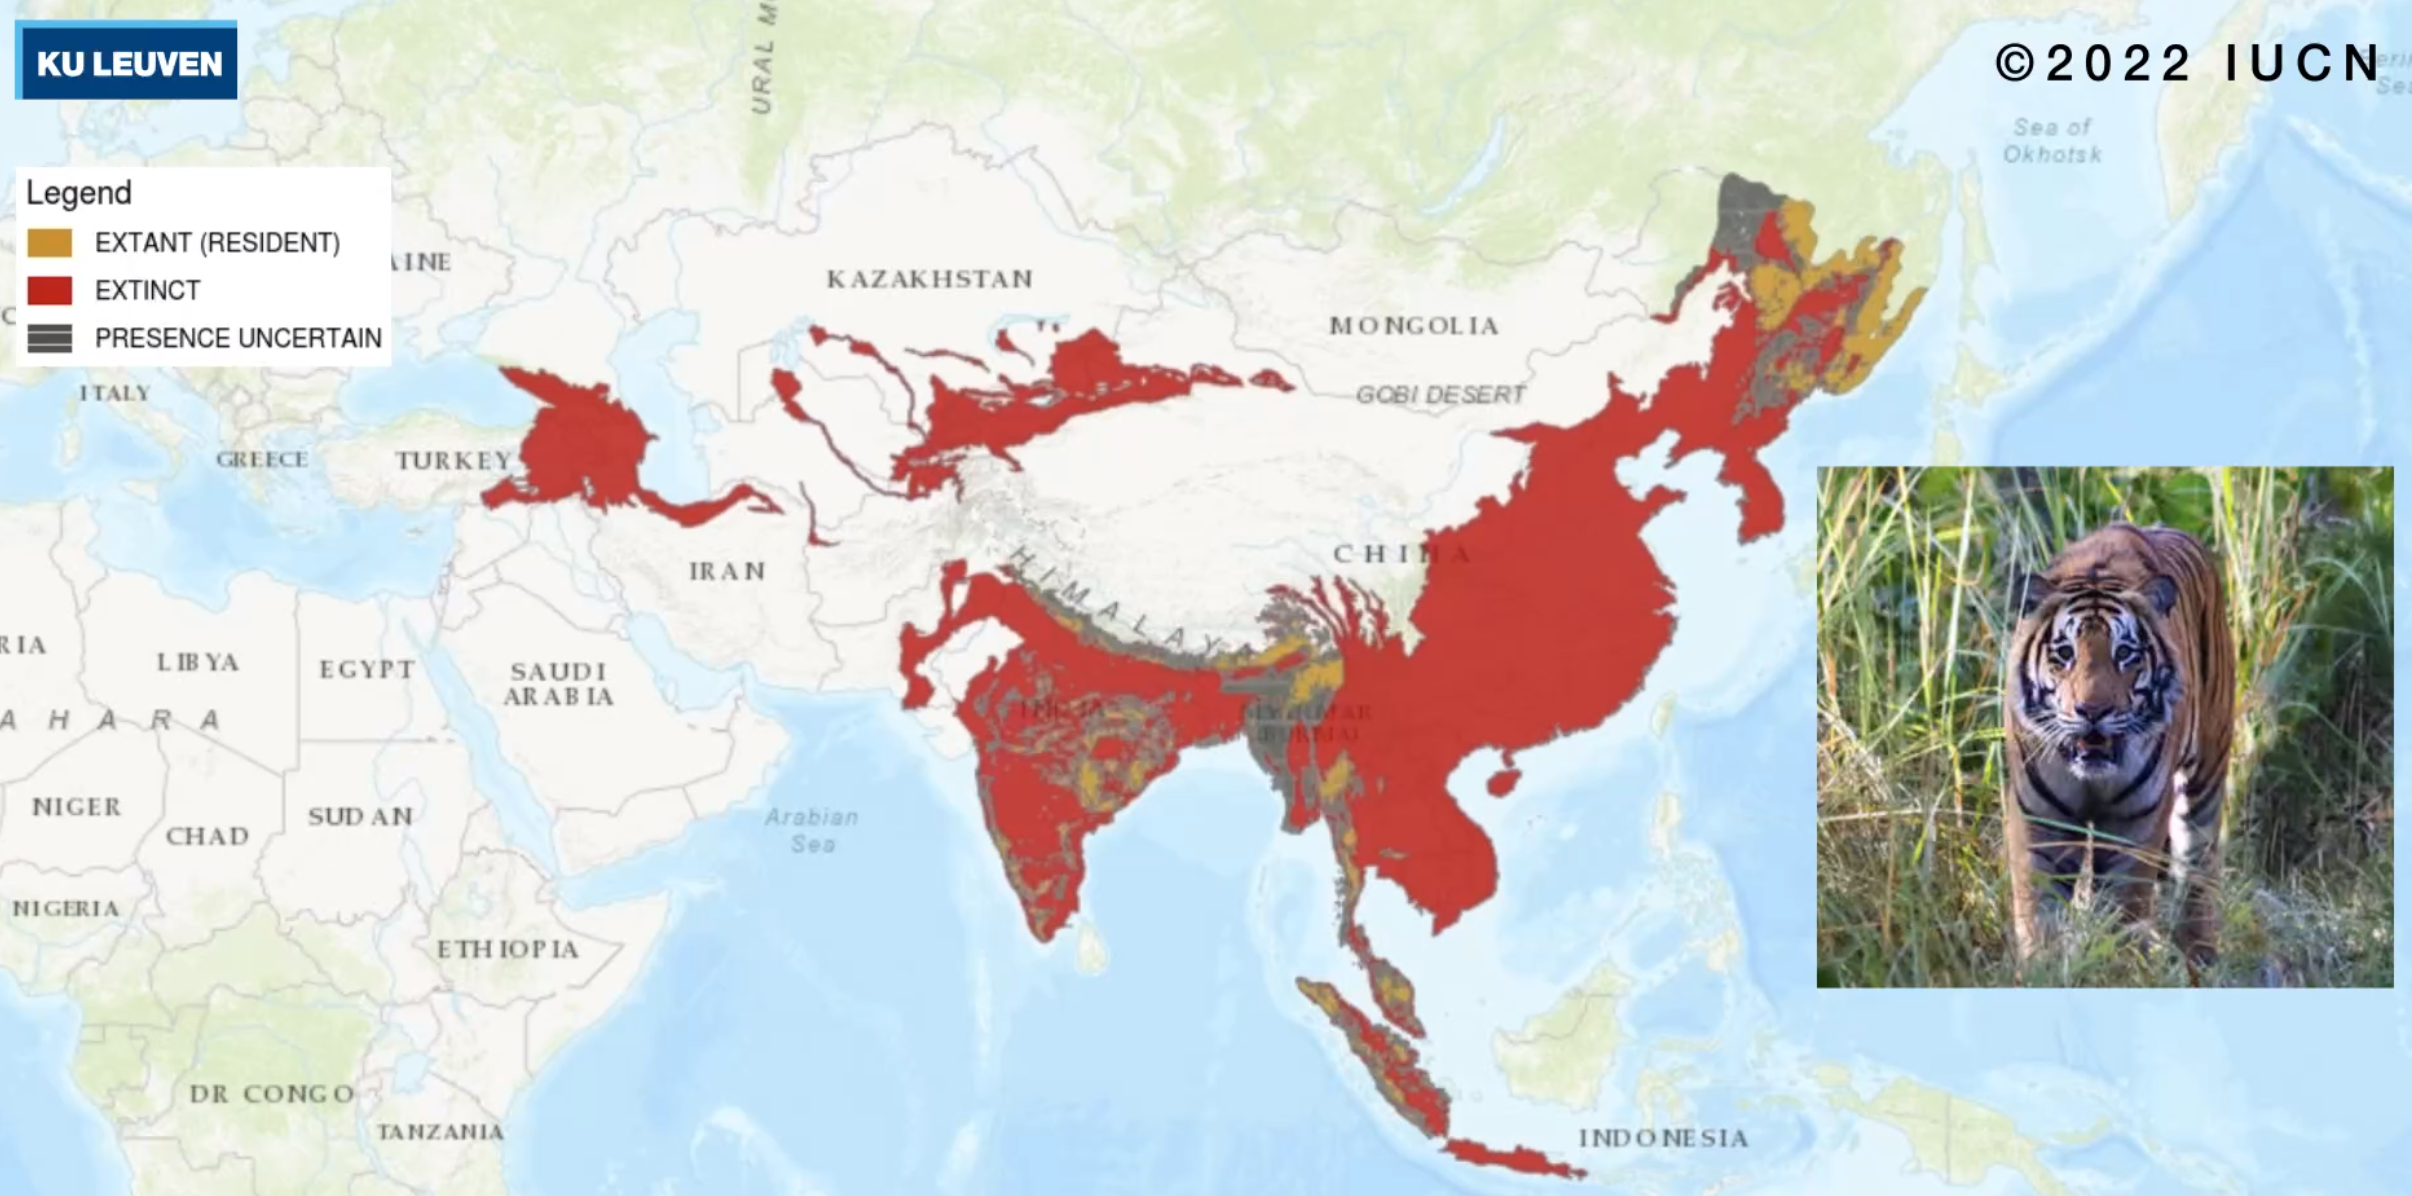
\includegraphics[width=0.9\linewidth]{../images/tiger_population}
	\caption{Tiger population in Asia}
	\label{fig:tigerpopulation}
\end{figure}
\ \\
The Living Planet Index (LPI) [figure \ref{fig:livingplanetindex}] shows the evolution of the average population size of 21 thousand animal populations around the globe. It shows a decline of 68\% since it's start in 1970. Keep in mind that the LPI is strongly influenced by a minority of populations with a very strong decrease in numbers [figure \ref{fig:lpi}].

\begin{figure}[H]
	\centering
	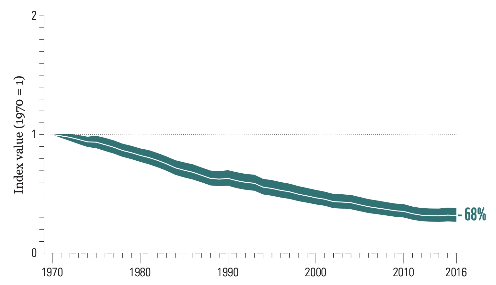
\includegraphics[width=0.8\linewidth]{../images/living_planet_index}
	\caption{The Living Planet Index}
	\label{fig:livingplanetindex}
\end{figure}

\begin{figure}[H]
	\centering
	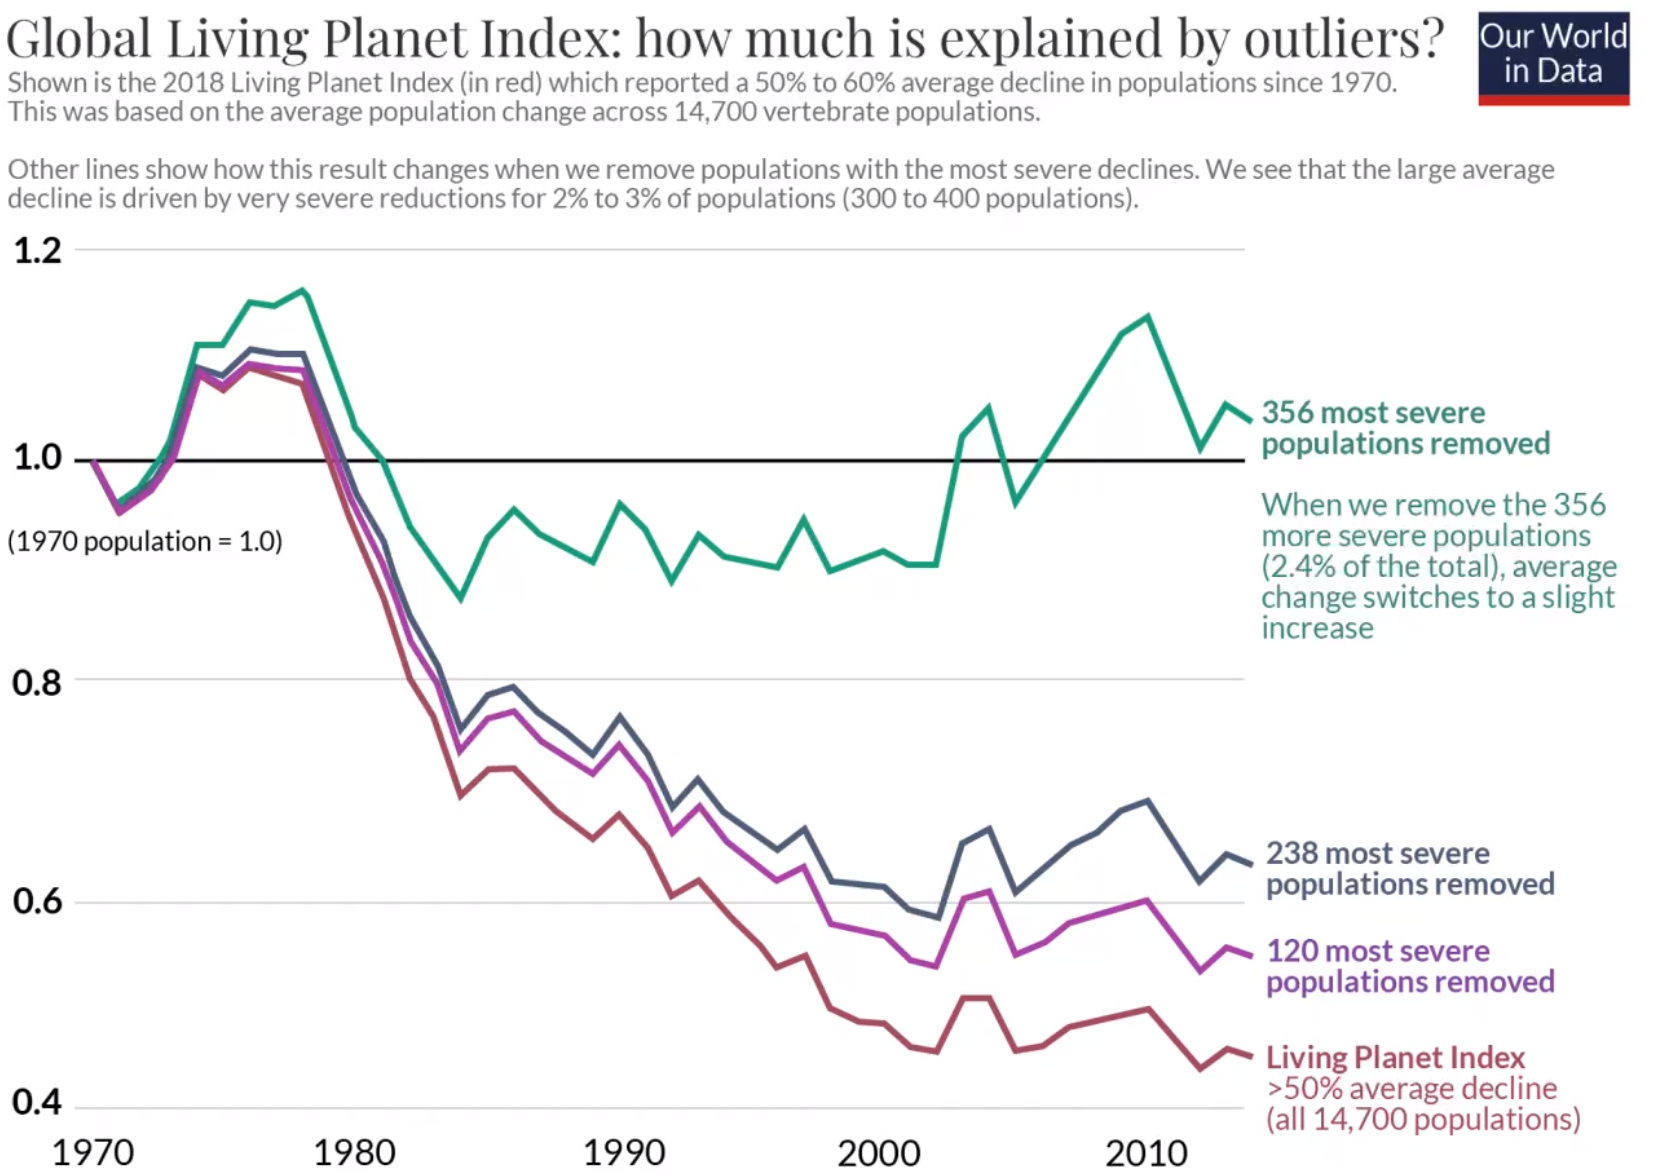
\includegraphics[width=0.8\linewidth]{../images/LPI}
	\caption{Impact of most severe declines on the Living Planet Index}
	\label{fig:lpi}
\end{figure}
\ \\
The IUCN Red List is another important monitoring program which monitors the extinction risk of individual species. Based on some criteria, species are assigned to one of the six classes on the list. The tiger for example is classified as endangered. In 2022, the IUCN identified 28\% of 150 thousand evaluated species to be threatened with extinction. 

\begin{figure}[H]
	\centering
	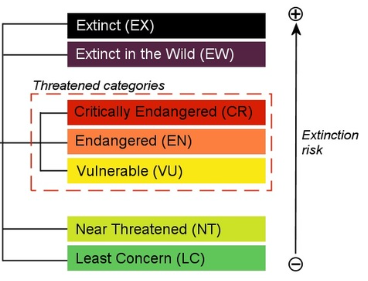
\includegraphics[width=0.6\linewidth]{../images/IUCN}
	\caption{The different classes of the IUCN Red List}
	\label{fig:iucn}
\end{figure}
\ \\
The IBPES, the Intergovernmental Science-Policy Platform on Biodiversity, concluded that 1 million of species on Earth are threatened with extinction.

\subsubsection{How to measure biodiversity loss?}

Measuring biodiversity loss is complex and requires

\begin{itemize}
	\item evidence of a clear \textbf{causal relationship }between intervention and impact: you have to be sure that the change in biodiversity is caused by the human intervention you are studying
	\item the \textbf{absence of other confounding factors}: you have to be sure that the human intervention is the only thing influencing the biodiversity
	\item and clear decisions on \textbf{which elements of biodiversity are considered}: biodiversity has many different components, so it’s important to define which components will be measured and how
\end{itemize}
 \ \\
 It requires simplified proxies like indicator species, which are known to be sensitive for certain human-induced disturbances,  or multi-taxa approaches, to sense the impact on different groups of organisms. Various techniques are used to measure different dimensions of biodiversity, including satellites, eDNA, camera traps, and citizen science.\\
 \\
 The IUCN Red List and the Living Planet Index are major indicator tools for global biodiversity loss, as seen in section \ref{sec:recent-diversity-loss}.
\\
\\
Mid-point indicators measure the frequency and intensity of damaging interventions, assuming a known relationship between intervention and effect. They are cheaper and have better data availability than measuring biodiversity effects itself. This approach is typical for Land Use Impact methods used in Life Cycle Assessment and Environmental Footprint Analysis, which calculate the impact of land use change (e.g. deforestation) or of permanent land use (e.g. long-term cropland) by measuring the loss of land quality over time for a certain area.  \\
(Land use change $\leftrightarrow$ Strong decline in small period | Permanent land use $\leftrightarrow$ less strong decline for a long period)

\begin{figure}[H]
	\centering
	
\includegraphics[width=0.5\linewidth]{../images/mid_point_indicator}
	\caption{Mid-point indicator}
	\label{fig:midpointindicator}
\end{figure}
\newpage

\subsection{Importance of biodiversity}
\subsubsection{Ecosystem services}

Biodiversity, the variety of life on Earth, has gained recognition for its vital role in sustaining human well-being. In the past, it was undervalued, leading to a biodiversity crisis. Robert Costanza proposed a shift from an "empty world model" to a "full world model," emphasizing the importance of biodiversity and other natural capital as a source of human prosperity and well-being..\\
\\
Ecosystem services, including provisioning, regulating, and cultural services, are the goods and services humans get from ecosystems. Biodiversity influences ecosystem functions like photosynthesis, evapotranspiration and nutrient cycling, which, in their turn, support a bundle of ecosystem services and enhance human prosperity. this is visualized in the Ecosystem Services Cascade (figure \ref{fig:ecosystemservicescascade}).

\begin{figure}[H]
	\centering
	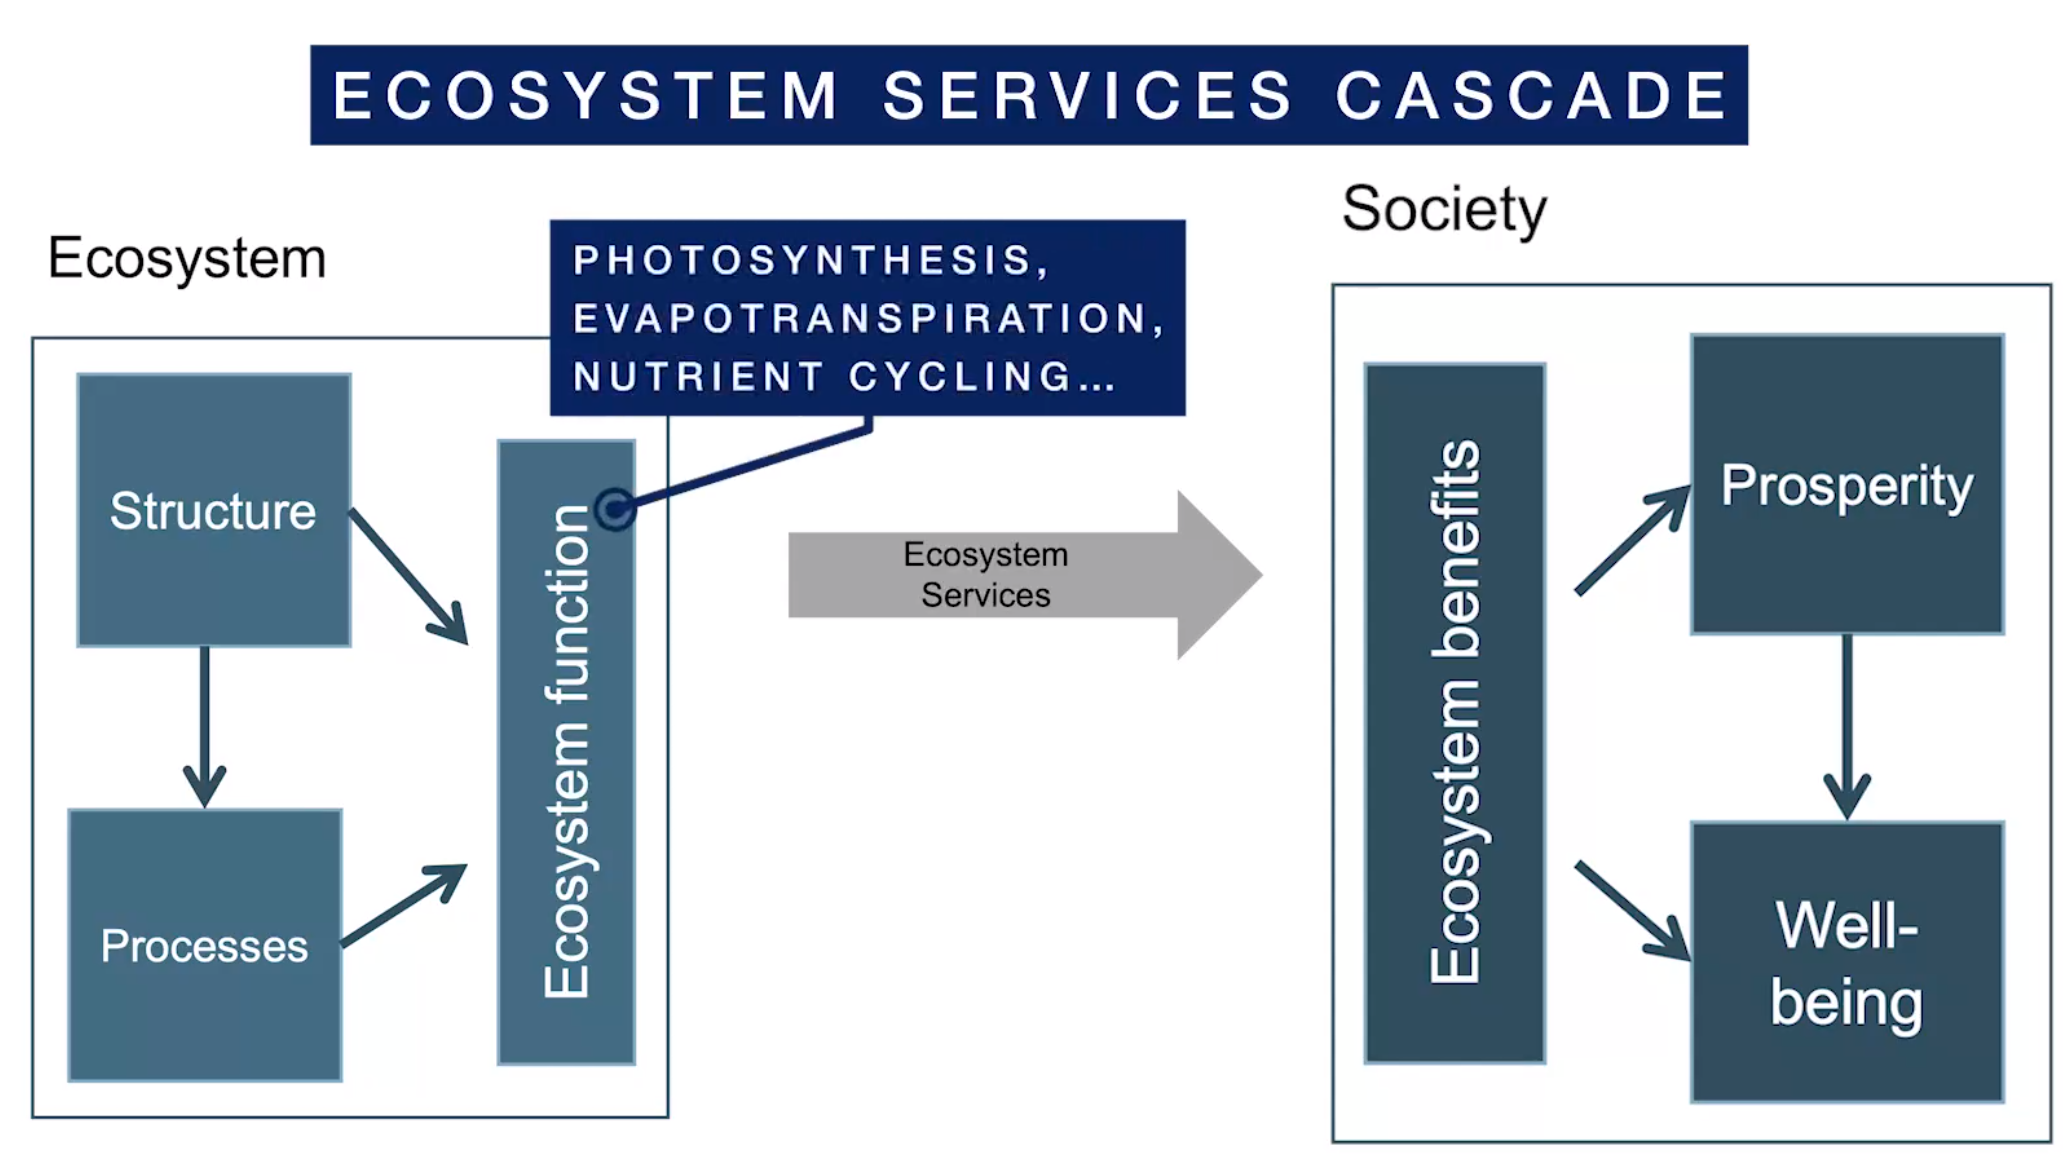
\includegraphics[width=0.6\linewidth]{../images/ecosystem_services_cascade}
	\caption{Ecosystem Services Cascade}
	\label{fig:ecosystemservicescascade}
\end{figure}
\ \\
\textbf{Provisioning services }$\leftrightarrow$ material flows, like agricultural crops for food, wood for construction, biomass for energy or drinking water.\\
\\
\textbf{Regulating services }$\leftrightarrow$ provide environmental protection like erosion control, air cooling and filtering by vegetation or climate mitigation through carbon uptake and storage in forests, peatlands and soils.\\
\\
\textbf{Cultural services} $\leftrightarrow$ provide diverse spiritual, recreational and scientific experiences ecosystems  to humans.
\\
\\
All these services directly depend on biodiversity. No food without crop species, no urban climate regulation without trees, no wilderness experience without vibrant ecosystems.\\
\\
Research shows that biodiversity positively affects ecosystem service performance, but there is a threshold beyond which additional biodiversity doesn't significantly increase service provision (figure \ref{fig:ecosystemserviceperformance1} and \ref{fig:ecosystemserviceperformance2}). Ecosystem degradation may not immediately lead to service losses, but crossing a critical species loss threshold can result in substantial reductions in services (figure \ref{fig:ecosystemserviceperformance3}).

\begin{figure}[H]
	\centering
	\begin{subfigure}[b]{0.4\textwidth}
		\centering
		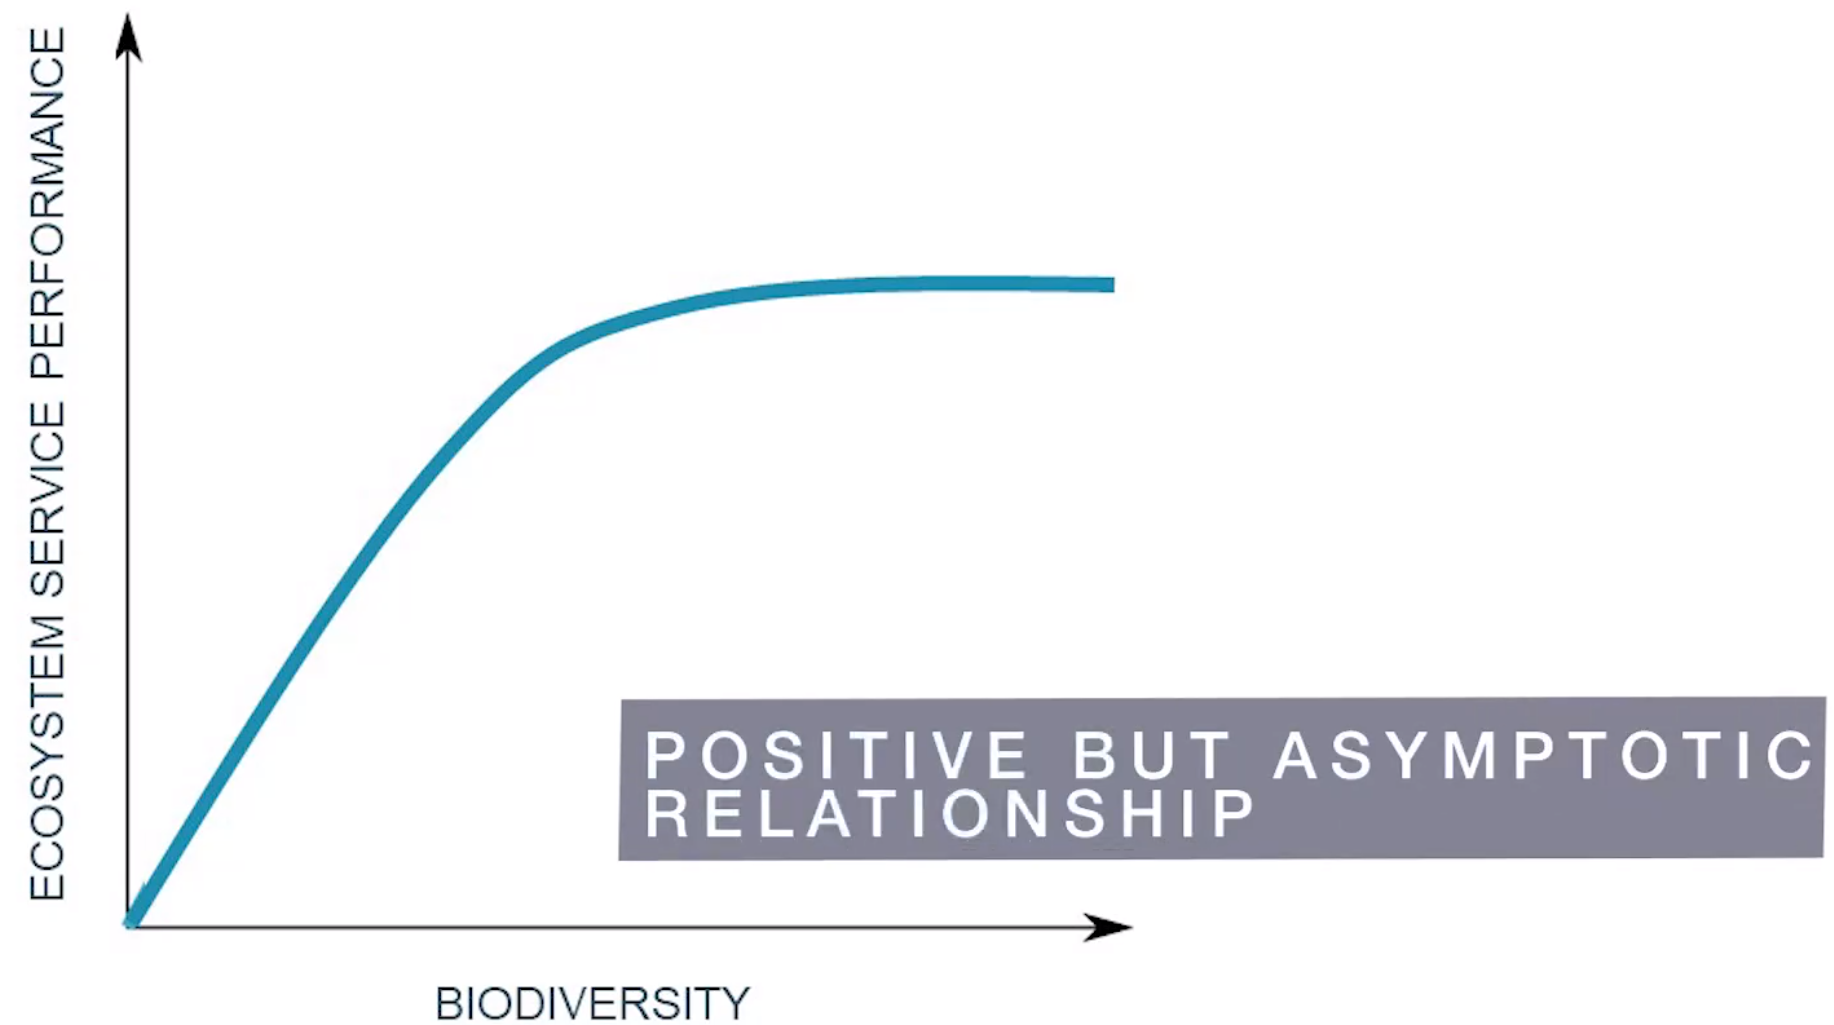
\includegraphics[width=\textwidth]{../images/ecosystem_service_cascade_1.png}
		\caption{}
		\label{fig:ecosystemserviceperformance1}
	\end{subfigure}
	\hfill
	\begin{subfigure}[b]{0.25\textwidth}
		\centering
		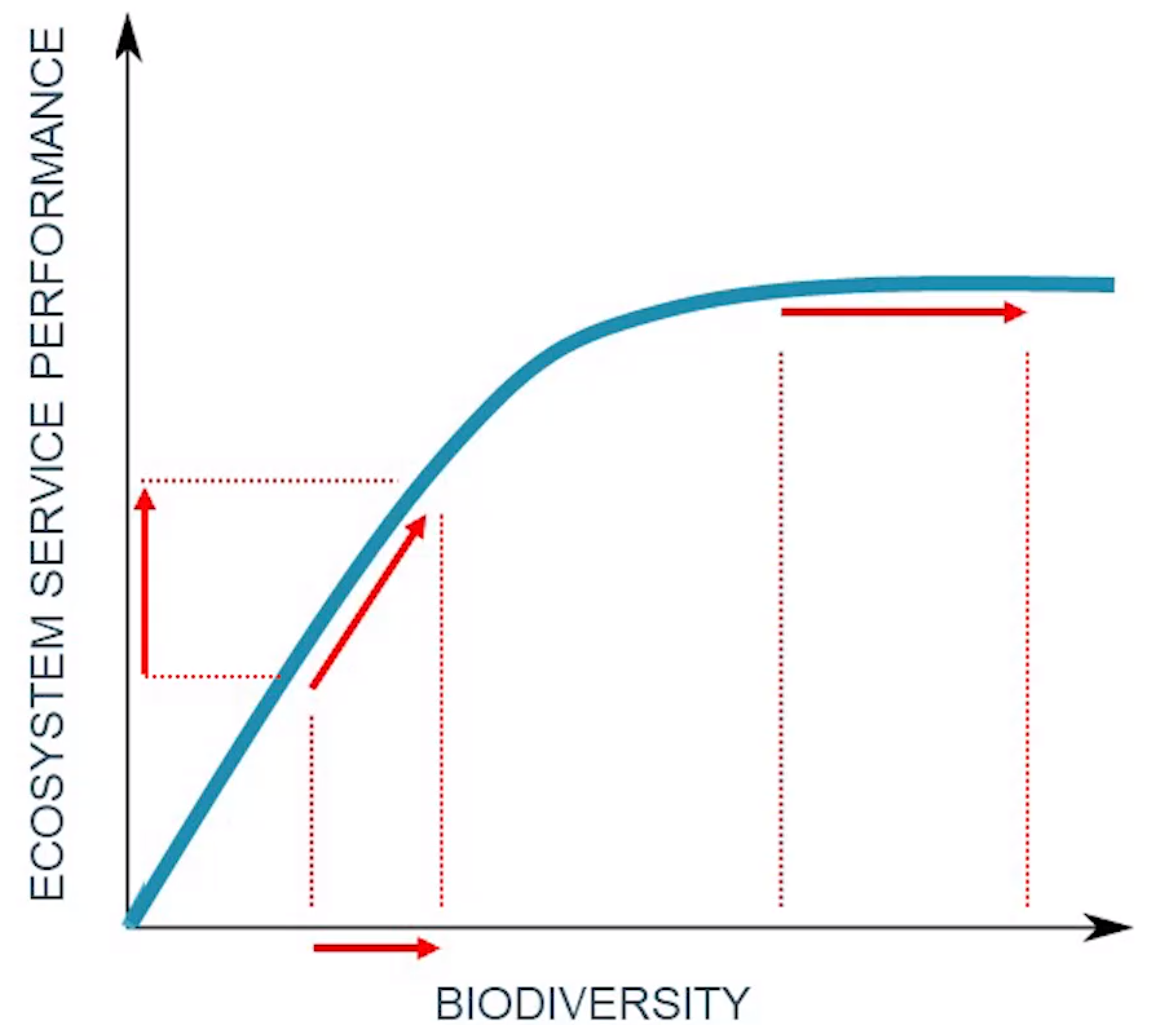
\includegraphics[width=\textwidth]{../images/ecosystem_service_cascade_2.png}
		\caption{}
		\label{fig:ecosystemserviceperformance2}
	\end{subfigure}
	\hfill
	\begin{subfigure}[b]{0.25\textwidth}
		\centering
		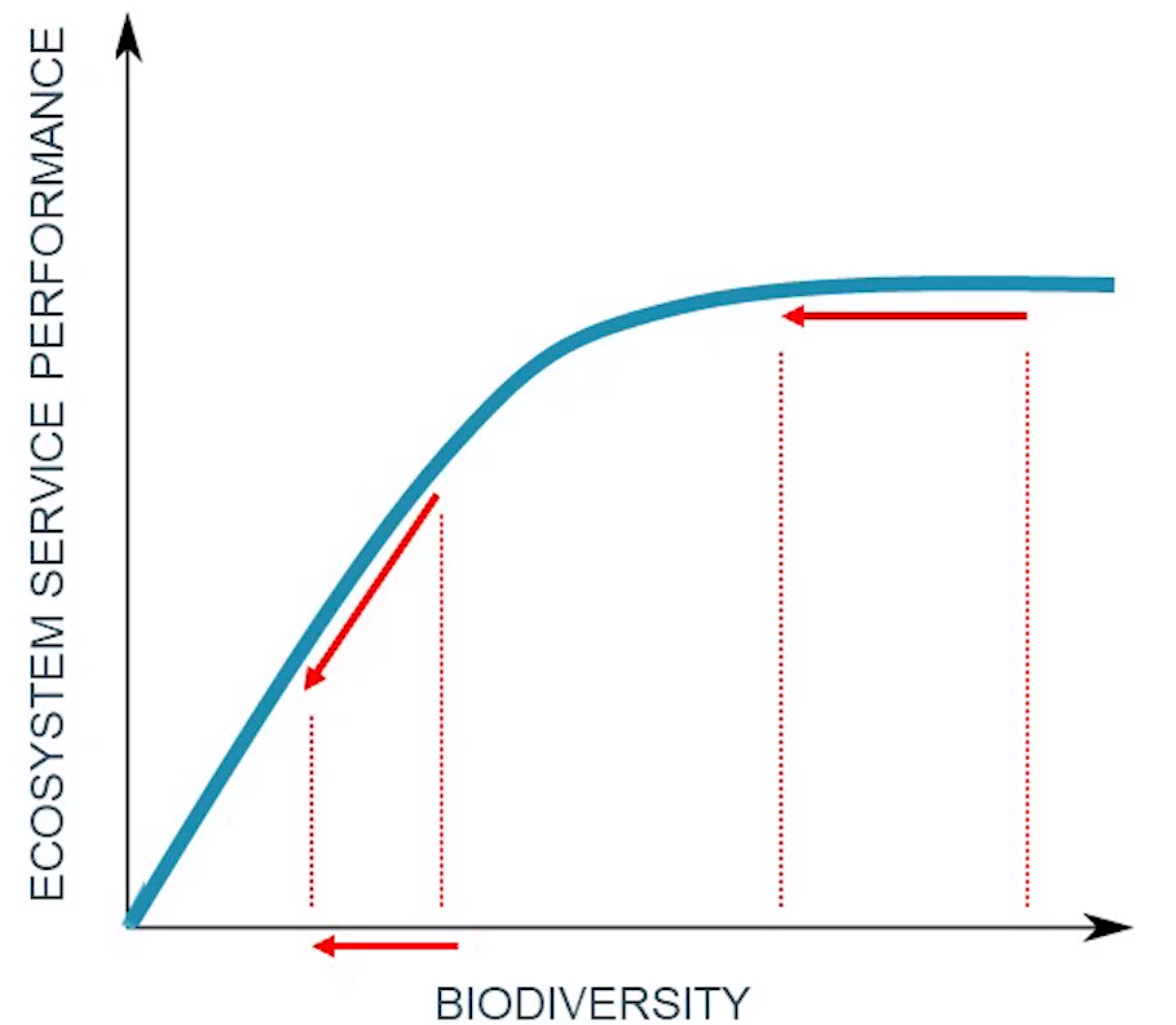
\includegraphics[width=\textwidth]{../images/ecosystem_service_cascade_3.png}
		\caption{}
		\label{fig:ecosystemserviceperformance3}
	\end{subfigure}
	\caption{Ecosystem service performance}
	\label{fig:ecosystemserviceperformance}
\end{figure}

\ \\
Biodiversity, more than just a heritage to protect, serves as a fundamental asset in the ecosystem service cascade, essential for human survival. The concept of "Nature's Contributions to People" recognizes the broader impact of living nature on human well-being, capturing both positive and negative aspects of this relationship.

\subsubsection{Example: Crop wild relatives}

Crop Wild Relatives (CWRs) are wild plant species genetically related to cultivated crops and provide a valuable \textbf{provisioning ecosystem service}. Over thousands of years, crops have been domesticated from their wild relatives, but this process reduced genetic diversity. CWRs continue to develop traits such as drought tolerance and pest resistance in the wild, offering opportunities for farmers and breeders to \textbf{create new and better adapted crop varieties by crossing the CWRs with domesticated crops}.\\
\\
CWRs have played a crucial role in overcoming challenges like the "grassy stunt virus" in rice. Over the last three decades, over 60 wild plant species have contributed genes to enhance the 13 most cultivated crops, improving their resilience to issues like drought and pests. \textbf{The introduction of wild relatives of our crops has contributed to about 30\% of the increase in crop yields since 1945.}\\
\\
\textbf{Conservation of crop wild relatives (CWRs) is of utmost importance} for enhancing crop production against emerging threats, but \textbf{many CWRs are at risk due to habitat destruction} caused by agricultural expansion. Ex situ conservation, storing CWRs outside their natural habitats in seed banks, offers a solution, with the Svalbard Global Seed Vault as a prominent example. However, ex situ conservation has limitations, as it may prevent CWRs from adapting to changing environmental conditions. Additionally, 95\% of CWRs are not adequately represented in gene banks, which means the full range of geographic and ecological variation in their native distribution is not covered.

\begin{figure}[H]
	\centering
	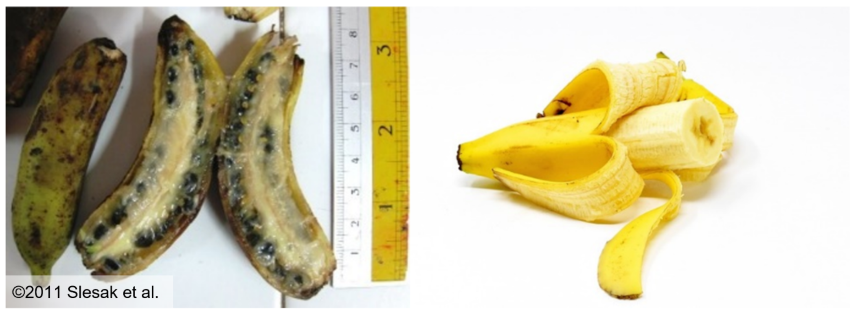
\includegraphics[width=0.7\linewidth]{../images/Banana_CWR_and_domesticated}
	\caption{CWR (Left) and the domesticated crop (Right) of a banana}
	\label{fig:bananacwranddomesticated}
\end{figure}
\newpage

\subsubsection{Example: Pollination}

Pollination, a \textbf{regulating ecosystem service} facilitated by biodiversity, is crucial for the reproduction of many agricultural crops. About \textbf{87 out of 124 major agricultural crops globally} (representing 35\% of the total agricultural production volume) \textbf{rely on insect pollination}. pollinating insects play a critical role in transferring pollen, leading to fertilization and seed and fruit development.\\
\\
Crops like apples, cocoa, almonds, and Robusta coffee depend on pollinators, while for others like Arabica coffee and rapeseed, they can enhance yields. However, crops such as wheat and maize do not need pollination.\\
\\
Globally, the value of pollinators for agricultural crops is significant, amounting to €153 billion annually, equivalent to 10\% of total agricultural production. Research indicates that \textbf{the diversity and abundance (the total number of individuals) of pollinators in agricultural fields positively relate to crop yield}. For example, coffee plantations near natural vegetation show higher pollinator richness and abundance, resulting in better coffee pollination and increased yields. Similar effects are seen in crops like apples and rapeseed.\\
\\
Notably, the effect of pollinators on crop production is influenced not only by their abundance but also by their \textbf{species richness}. The complementarity effect ensures that different pollinator species have optimal conditions for pollination, making it crucial to increase pollinator species richness through conservation efforts, such as establishing flower strips or small landscape elements in agricultural landscapes. These actions help maintain or enhance yields of insect-pollinated crops.

\subsection{Evil Quintet}
\subsubsection{Overview}
Biodiversity is under threat, with biosphere integrity being a planetary boundary breach. The main threats to biodiversity are categorized into five drivers in decreasing order of importance: \textbf{habitat loss, overexploitation through hunting and fishing, climate change, pollution, and invasive species}. These five drivers are called the Evil Quintet. \\
\\
Habitat loss is mainly caused by expanding agricultural land, particularly in tropics and subtropics. Overexploitation occurs for food or valuable body parts like ivory. Climate change is a new threat, with species hampered by habitat loss. Pollution is caused by agrochemicals and overuse of fertilizers. Invasive species may outcompete or predate indigenous species. Other threats include wildfires and human disturbances.

\subsubsection{Habitat loss and degradation}

Habitat loss is the primary driver of biodiversity loss worldwide, with the main cause being the conversion of natural ecosystems into agricultural land, which are very active in South America, Sub-Saharan Africa, and South-East Asia. Among 703 declining terrestrial populations, habitat loss contributes to 50\% of the threats, followed by overexploitation at 25\%, invasive species at 10\%, and climate change and pollution at 7-8\% each (figure \ref{fig:biodiversitythreats}).\\
\\
Notably, agriculture already covers 50\% of inhabitable terrestrial area, with over 75\% of this used for livestock, which can be energetically inefficient for food production. The loss of forest cover is ongoing at a rapid rate of about 20 million hectares per year, resulting in a gross loss of 3.6 million square kilometres from 2001-2018, with a significant portion converted to agriculture.

\begin{figure}[H]
	\centering
	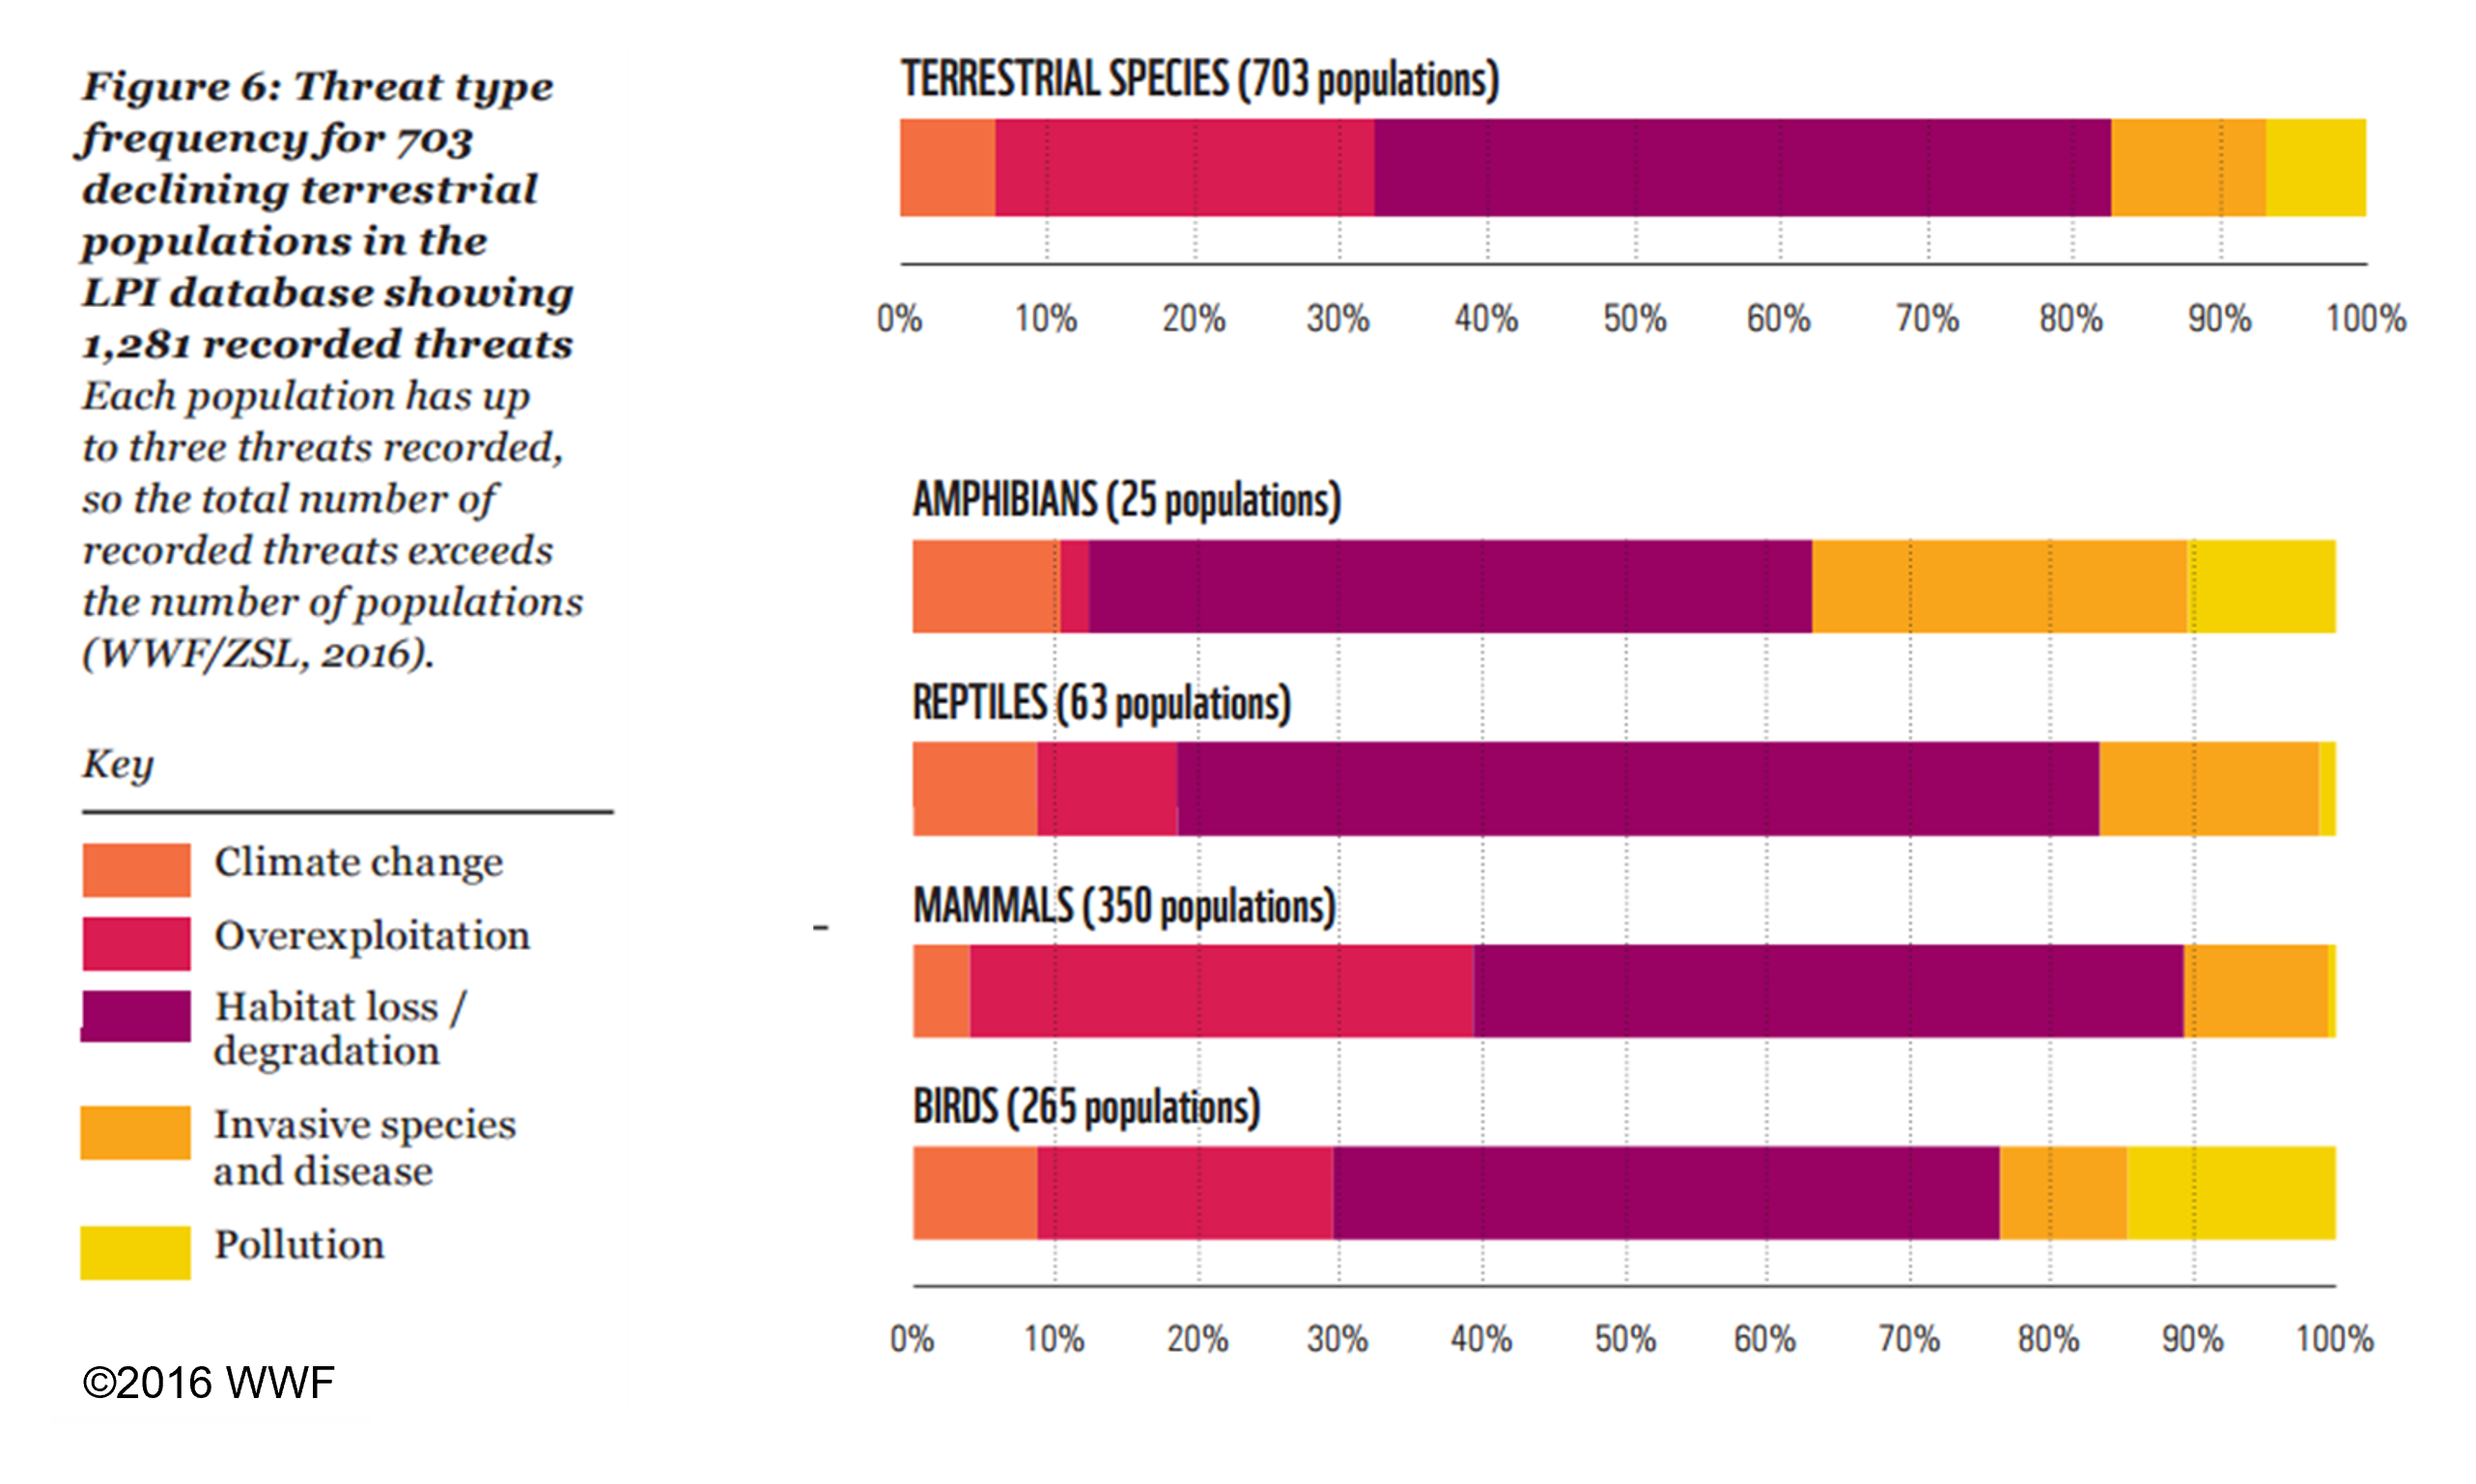
\includegraphics[width=0.65\linewidth]{../images/Biodiversity_threats}
	\caption{Threats of different species}
	\label{fig:biodiversitythreats}
\end{figure}

\subsubsection{Overexploitation}

Overexploitation is a key contributor to biodiversity loss, occurring when plant and animal populations are excessively harvested. To ensure sustainability, harvesting must remain below natural population growth, requiring strict monitoring and governance. Sustainable models exist in sectors like fisheries, game hunting, and responsible forest use.\\
\\
Weak governance often leads to overexploitation, harming wildlife populations. Historically, larger vertebrates like bison, whales, beavers, and rhinos have been exploited for their valuable attributes, including meat, fat, and fur. Among the 362 megafauna species on Earth, overexploitation is a major threat, as shown in a figure.

\begin{figure}[H]
	\centering
	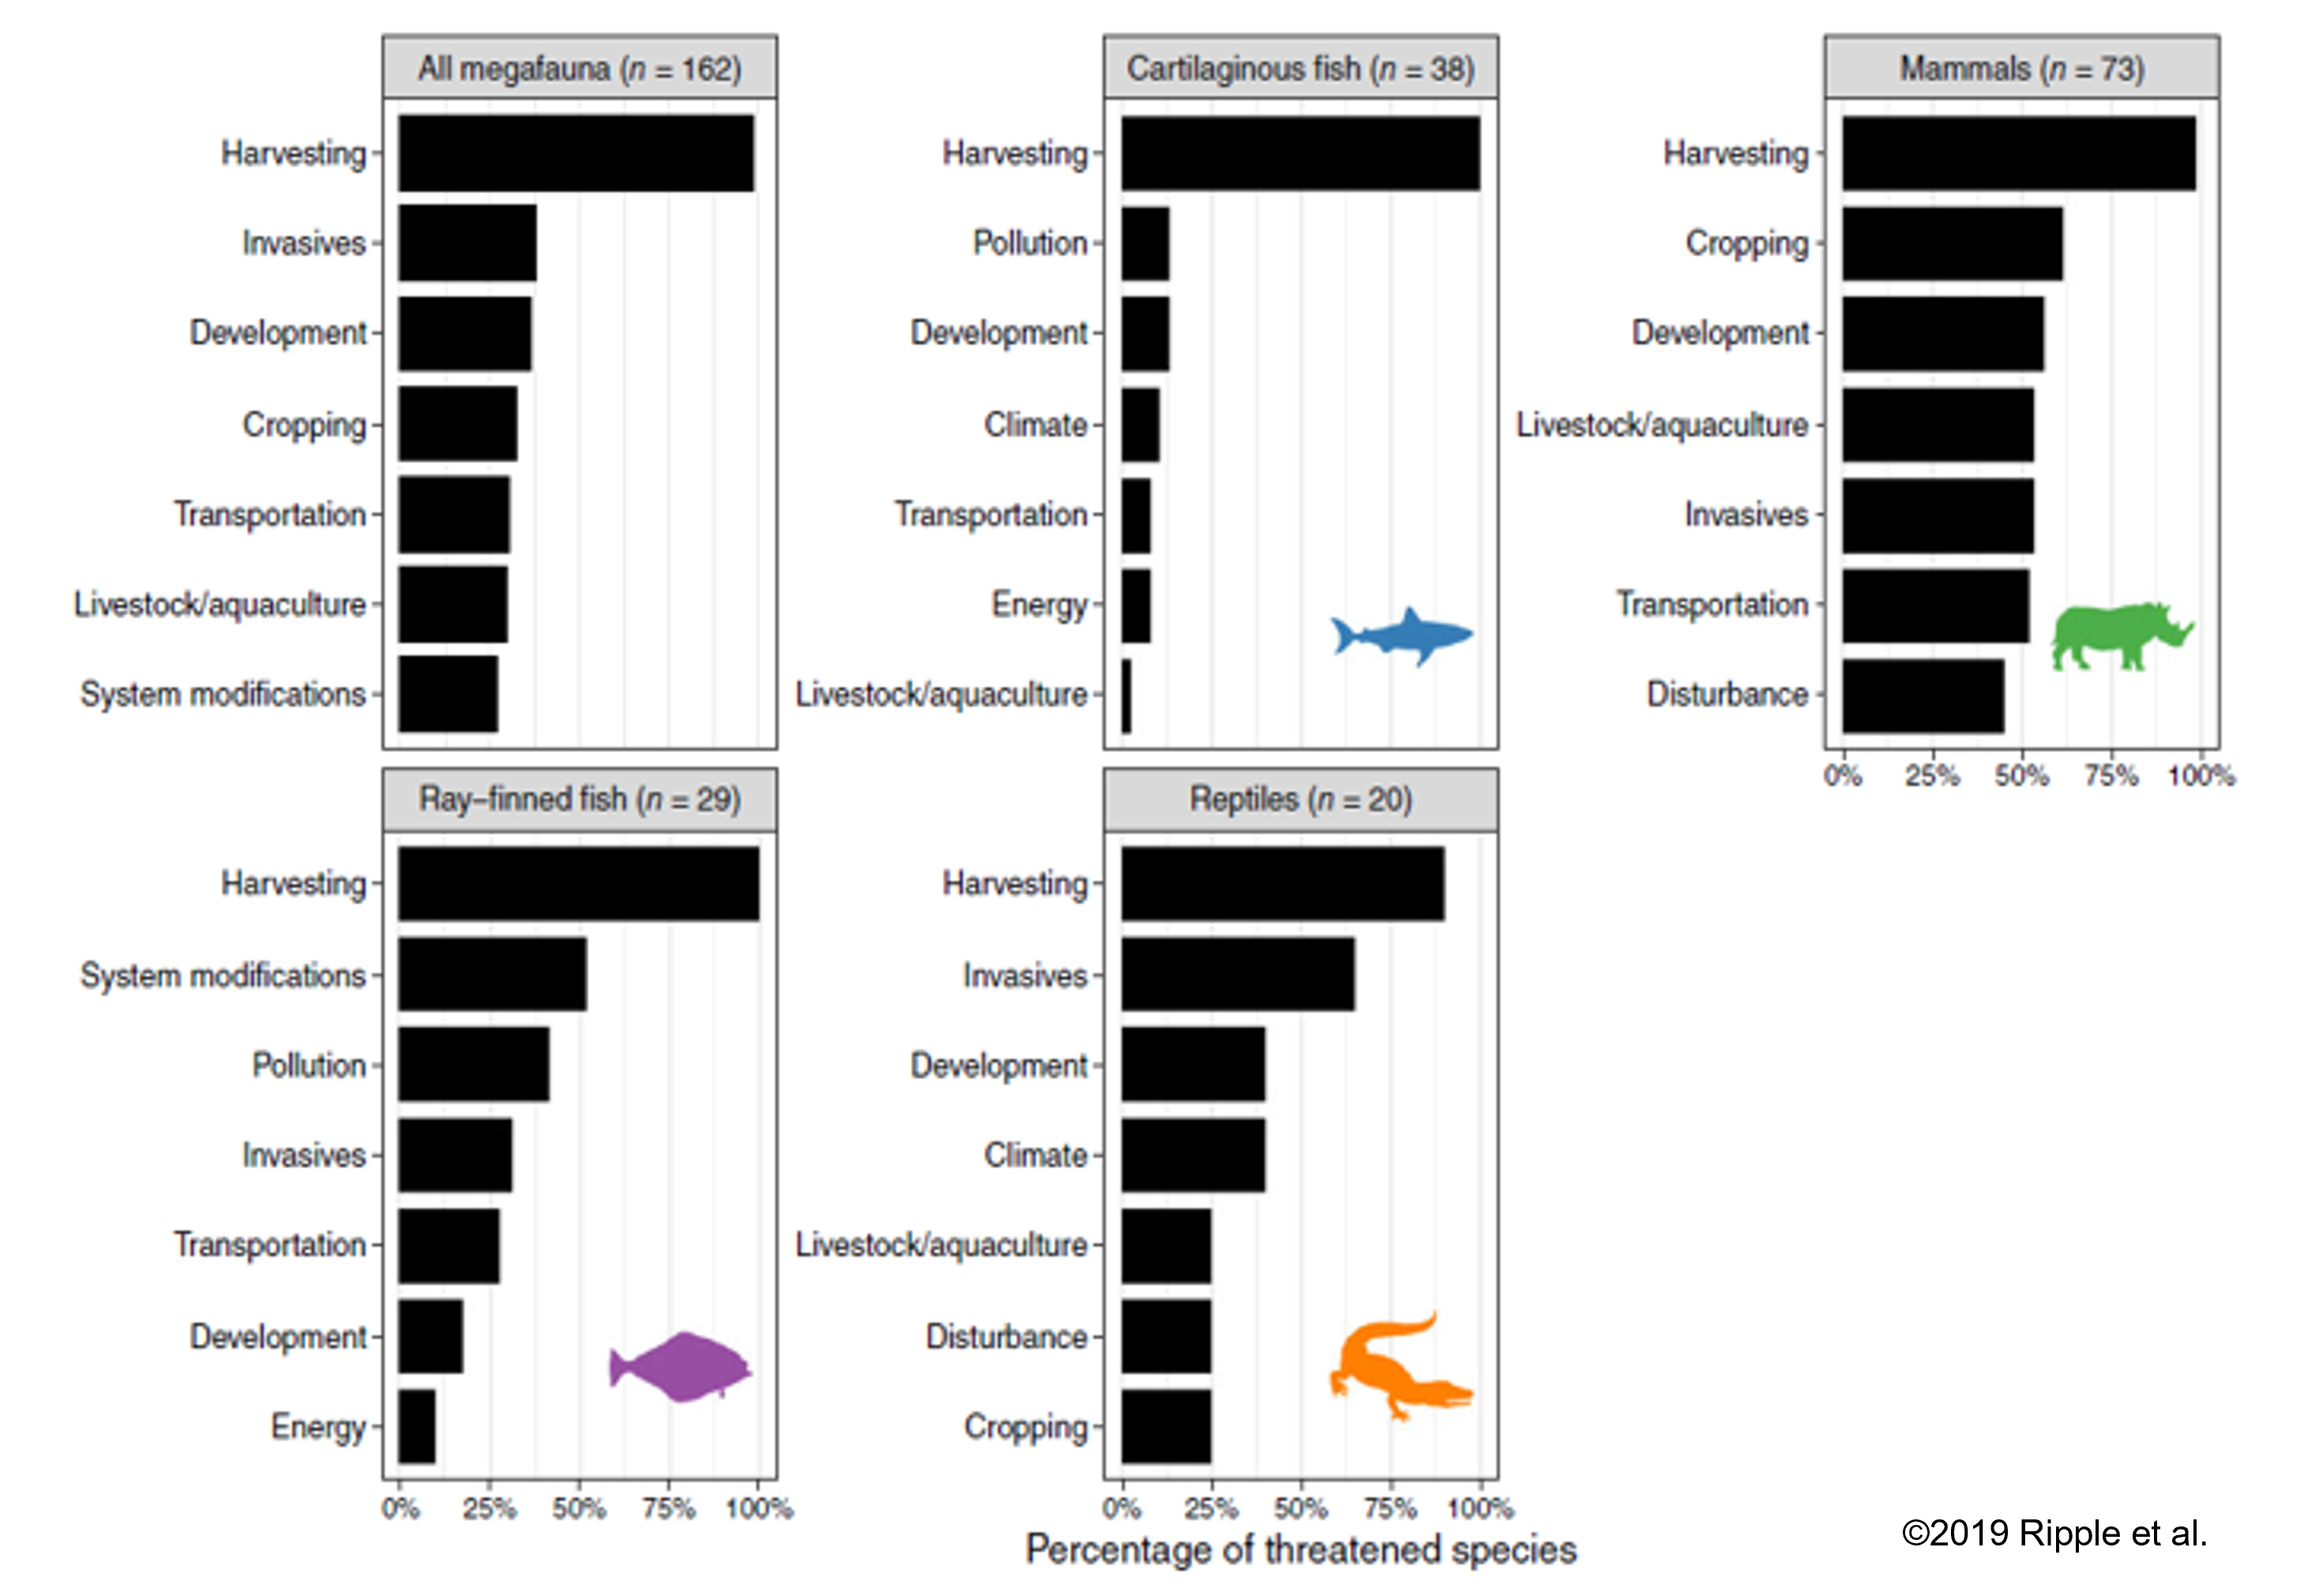
\includegraphics[width=0.65\linewidth]{../images/Share_of_overharvesting}
	\caption{Percentage of threatened species}
	\label{fig:shareofoverharvesting}
\end{figure}


\ \\
The bushmeat market in West Africa exemplifies overexploitation, transforming tropical forests into "silent" zones. All eight pangolin species worldwide are threatened by overexploitation. Additionally, these markets pose the risk of zoonotic disease transmission from animals to humans. Pangolins, for instance, may have played a role as intermediate hosts for zoonotic diseases like Covid-19, transferring from bats to humans.

\subsubsection{Invasive species}
\paragraph{What are invasive alien species?}
\ \\\\
\textbf{Alien} (or exotic or non-native) \textbf{species} are species that are introduced by humans, accidentally or intentionally, outside of their natural geographic range into an area where they were not naturally present. This as opposed to \textbf{indigenous} (or native) \textbf{species}. A species is indigenous to a given region or ecosystem if its presence in that region is the result of only natural processes, with no human intervention. \\
\\
\textbf{Invasive alien species} (IAS) are non-native species that cause economic or environmental harm or adversely affect human health. It is important to note that not all alien species cause harm and are thus classified as invasive. 

\paragraph{How are alien species introduced?}
 \ \\\\
 Alien species can be introduced in many ways. Usually we divide them into \textbf{unintentional/accidental} and \textbf{intentional} introductions. Not all of these imported species become invasive, but sometimes they do and start causing harm to the environment, economy and/or human health. Let's look at some examples of introduction pathways.
 
 \begin{figure}[H]
 	\centering
 	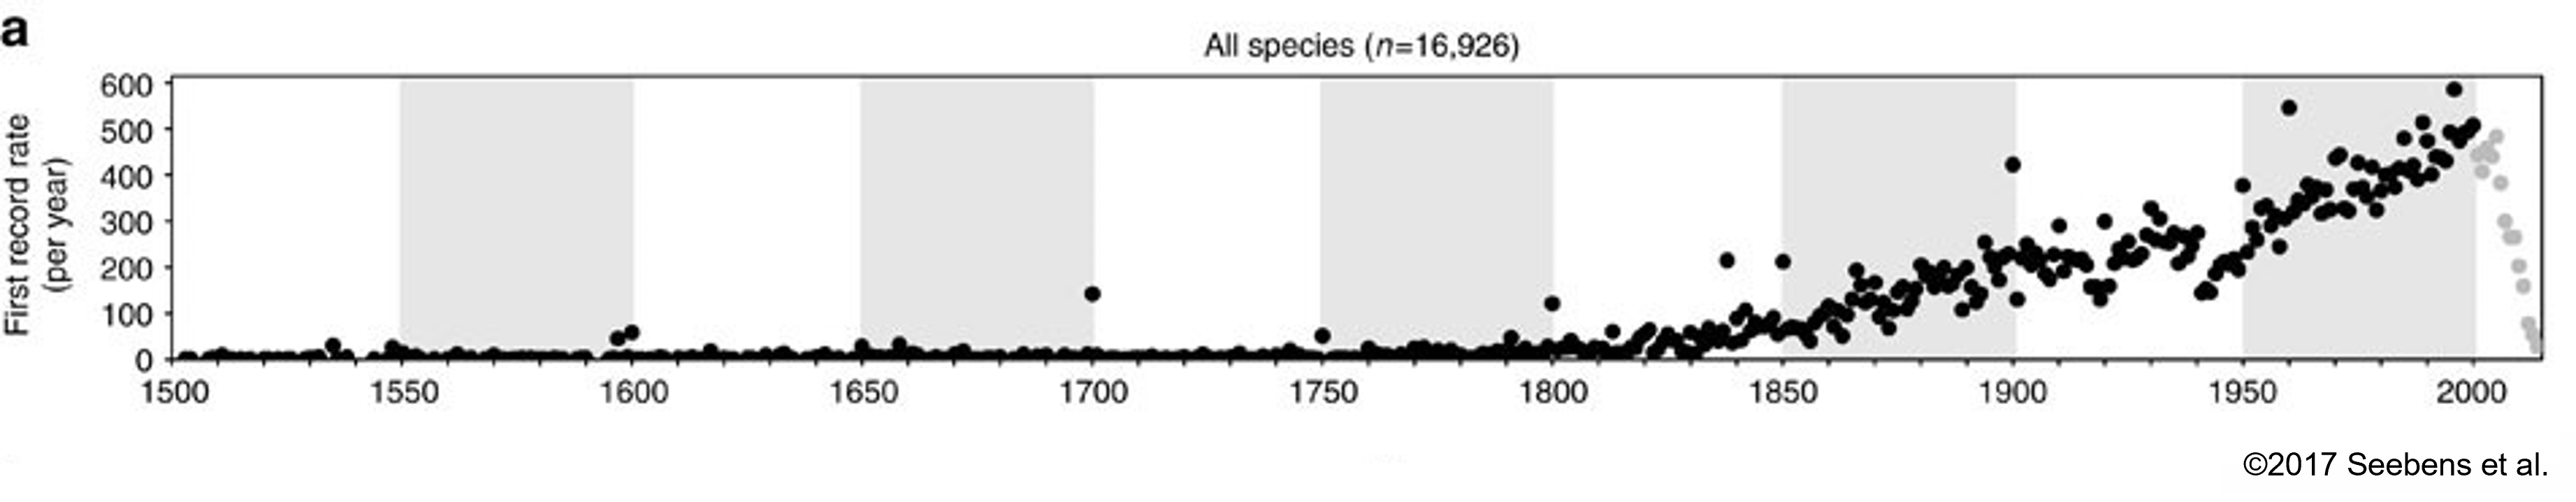
\includegraphics[width=0.8\linewidth]{../images/Alien_species_through_time}
 	\caption{Amount of new alien species recorded each year worldwide between 1500 and 2014}
 	\label{fig:alienspeciesthroughtime}
 \end{figure}
 \ \\
\underline{\textbf{ Accidental Introduction}}\\
  Three examples of accidental introduction are displayed in figure \ref{fig:accidentalintroduction}.
 
 \begin{figure}[H]
 	\centering
 	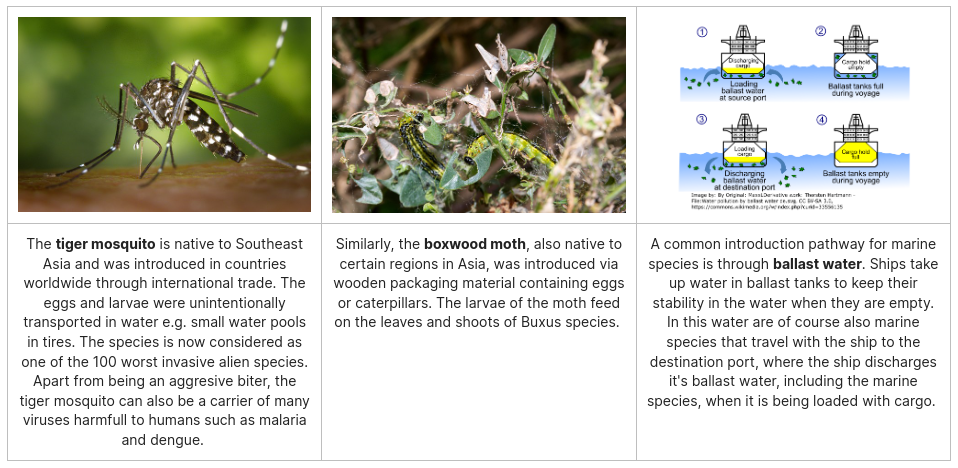
\includegraphics[width=0.9\linewidth]{../images/accidental_introduction}
 	\caption{Examples of accidental introductions}
 	\label{fig:accidentalintroduction}
 \end{figure}
 
 \newpage
 \ \\
 \underline{\textbf{ Inte ntional Introduction}}\\
There are many reasons why people brought (and still bring) alien species into a country:

\begin{itemize}
	\item \textbf{Ornamental plants}: Many plants are imported for their ornamental value for gardens, parks, etc... An example of a very invasive species is the Japanese knotweed.
	\item \textbf{Beekeeping}: for example Himalayan balsem was imported for the high nectar productivity, which is interesting for beekeeping.
	\item \textbf{Pets}: often animals are imported as pets, but then escape or are released into the wild, for example turtles that grow too large. 
	\item \textbf{Forestry}: some plants were introduced as an interesting species for forestry, but then became invasive, such as the Black cherry
	\item \textbf{Pest control}: for example the Asian lady beetle was introduced to control pests in greenhouses
\end{itemize}

\paragraph{Impact of invasive alien species}
 \ \\\\
\underline{Effects on native biodiversity}\\
\begin{itemize}
	\item \textbf{Predation}: e.g. the Asian lady beetle, which outcompetes and even eats other native lady beetles, or the American bull frog, which eats small birds, other amphibian species, fish, snails, insects, ...
	\item \textbf{Introduction of new diseases and pests}: e.g. the Horse-chestnut leaf miners are an invasive pest of horse chestnut leading to an early autumn browing, or the Varrao mite parasites on bees, which carry around several viruses that can contribute to the 'colony collapse disorder'.
	\item \textbf{Competition with native species}: e.g. Japanese knotweed, which has such a dominant growth it blocks the sunlight for other species, or the Himalayan balsam, which is a strong competitor for pollinators.
\end{itemize}
\ \\
\underline{Effects on humans}\\
Invasive species can also effect human health by many pathways. Here are some examples:
\begin{itemize}
	\item The tiger mosquito is a vector of many \textbf{viral pathogens}, including the yellow fever virus and dengue fever.
	\item The ragweed Ambrosia artemisiifolia has strong \textbf{allergenic} properties and is invasive in Europe. 
	\item Invasive alien species can pose a \textbf{threat to agriculture and forestry}, e.g. the Giant African snail introduced to North and South America.
\end{itemize}

\subsubsection{Pollution}



\end{document}